% ============================================================
%  VAPT Mini-Project Report — LeBlanc Pipeline
%  Compile: pdflatex vapt_report.tex  (twice for refs)
% ============================================================
\documentclass[11pt,a4paper]{article}

% ---------- packages ----------
\usepackage[T1]{fontenc}
\usepackage[utf8]{inputenc}
\usepackage{lmodern}
\usepackage[margin=2.4cm]{geometry}
\usepackage{microtype}
\usepackage{parskip}
\usepackage{titlesec}
\usepackage{booktabs}
\usepackage{array}
\usepackage{tabularx}
\usepackage{xcolor}
\usepackage{listings}
\usepackage{enumitem}
\usepackage{hyperref}
\usepackage{fancyhdr}
\usepackage{graphicx}
\usepackage{float}
\usepackage{tikz}
\usetikzlibrary{shapes.geometric, arrows.meta, positioning, fit, backgrounds}

% ---------- colours ----------
\definecolor{accent}{HTML}{1A3C5E}
\definecolor{lightgray}{HTML}{F4F6F8}
\definecolor{midgray}{HTML}{6B7280}
\definecolor{codegreen}{HTML}{22863A}
\definecolor{codebg}{HTML}{F6F8FA}
\definecolor{high}{HTML}{D73A49}
\definecolor{med}{HTML}{E36209}
\definecolor{low}{HTML}{2188FF}

% ---------- section styling ----------
\titleformat{\section}{\large\bfseries\color{accent}}{}{0em}{}[\titlerule]
\titleformat{\subsection}{\normalsize\bfseries\color{accent}}{}{0em}{}
\titlespacing{\section}{0pt}{18pt}{6pt}
\titlespacing{\subsection}{0pt}{10pt}{4pt}

% ---------- header / footer ----------
\pagestyle{fancy}
\fancyhf{}
\renewcommand{\headrulewidth}{0.4pt}
\fancyhead[L]{\small\color{midgray}LeBlanc — VAPT Mini-Project}
\fancyhead[R]{\small\color{midgray}April 2026}
\fancyfoot[C]{\small\thepage}

% ---------- code listing ----------
\lstset{
  backgroundcolor=\color{codebg},
  basicstyle=\ttfamily\footnotesize,
  breaklines=true,
  frame=single,
  rulecolor=\color{lightgray},
  commentstyle=\color{codegreen},
  keywordstyle=\bfseries,
  numbers=left, numberstyle=\tiny\color{midgray}, numbersep=6pt,
  xleftmargin=12pt, xrightmargin=4pt,
  captionpos=b,
}

% ---------- hyperref ----------
\hypersetup{colorlinks=true, linkcolor=accent, urlcolor=accent}

% ============================================================
\begin{document}

% ---- Title block ----
\begin{center}
  {\LARGE\bfseries\color{accent} Vulnerability Assessment \& Penetration Testing}\\[4pt]
  {\large\bfseries LeBlanc: Automated Security Analysis of LLM-Generated Code}\\[10pt]
  {\normalsize
    Suryanshu Banerjee \quad Vedant Walunj \quad Ritwik Mohanty}\\[4pt]
  {\small\color{midgray} Mini-Project Report \quad|\quad April 2026}
\end{center}
\vspace{-4pt}
\noindent\rule{\linewidth}{1pt}
\vspace{6pt}

% ============================================================
\section{Problem Statement}

Large Language Models (LLMs) such as Gemini and Llama are increasingly used by developers to generate production-ready Python code. However, empirical studies consistently show that LLM-generated code routinely introduces critical security flaws — SQL injection (CWE-89), path traversal (CWE-22), OS command injection (CWE-78), cross-site scripting (CWE-79), insecure file uploads (CWE-434), and weak cryptographic practices (CWE-328) — without any warning to the user.

\textbf{The core problem} is two-fold:

\begin{enumerate}[leftmargin=*, nosep]
  \item \textbf{Prompts carry no security context.} A developer asking an LLM to \textit{"write a Flask login endpoint"} receives syntactically correct but potentially injectable code because the model is not cued to apply secure-coding constraints.
  \item \textbf{No closed-loop correction exists.} Even when a vulnerability is detected post-generation, there is no systematic mechanism to feed scanner output back into the LLM and iterate until the code is clean.
\end{enumerate}

These gaps make LLM-assisted development a novel and understudied attack surface. Unlike traditional VAPT, which targets deployed infrastructure, this project addresses security \emph{at code-generation time} — before vulnerable code ever reaches a repository or production system.

% ============================================================
\section{Objectives}

\begin{enumerate}[leftmargin=*, label=\textbf{O\arabic*.}]
  \item \textbf{Identify vulnerability-prone LLM prompts.} Curate 10 representative prompts (P001–P010) spanning authentication, file access, command execution, session management, and cryptography — categories consistently associated with OWASP Top 10 and CWE Top 25 weaknesses.
  \item \textbf{Assess generated code using dual-tool static analysis.} Apply Semgrep and Bandit (medium-severity threshold) to LLM output, yielding CWE-mapped, line-level vulnerability reports.
  \item \textbf{Evaluate the impact of security-aware prompt enrichment.} Measure whether injecting CWE-specific warnings into the prompt (Engine A) reduces vulnerability count before any code repair.
  \item \textbf{Quantify iterative LLM-guided remediation.} Run up to five repair iterations (Engine C), feeding scanner findings back to the LLM, and track convergence to a clean state.
  \item \textbf{Compare two production LLMs.} Benchmark Gemini 2.5 Flash (Google AI) against Llama 3.3 70B (Groq) across all three pipeline modes to understand model-specific security behaviour.
\end{enumerate}

% ============================================================
\section{System Architecture}

\begin{figure}[H]
\centering
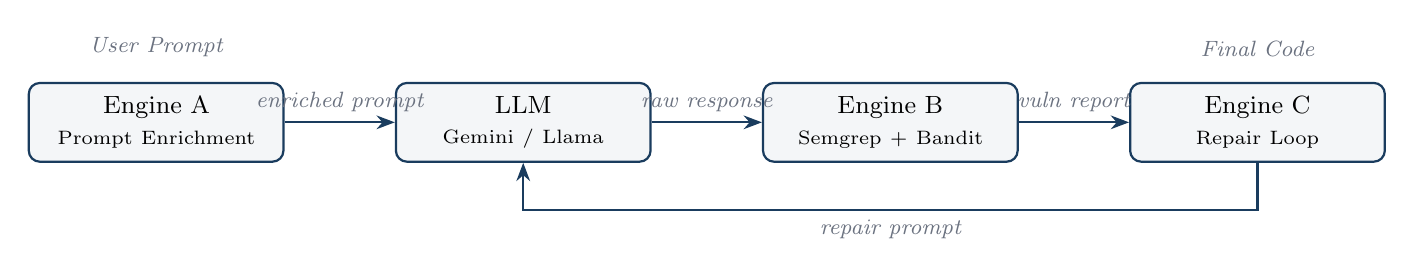
\begin{tikzpicture}[
  font=\small,
  box/.style={rectangle, rounded corners=4pt, draw=accent, thick,
              fill=lightgray, text width=3.0cm, align=center, minimum height=1cm},
  arrow/.style={-Stealth, thick, color=accent},
  label/.style={font=\footnotesize\itshape, color=midgray},
]

\node[box] (A) {Engine A\\{\scriptsize Prompt Enrichment}};
\node[box, right=1.4cm of A] (LLM) {LLM\\{\scriptsize Gemini / Llama}};
\node[box, right=1.4cm of LLM] (B) {Engine B\\{\scriptsize Semgrep + Bandit}};
\node[box, right=1.4cm of B] (C) {Engine C\\{\scriptsize Repair Loop}};

\draw[arrow] (A) -- (LLM) node[midway, above, label] {enriched prompt};
\draw[arrow] (LLM) -- (B) node[midway, above, label] {raw response};
\draw[arrow] (B) -- (C) node[midway, above, label] {vuln report};
\draw[arrow] (C.south) -- ++(0,-0.6) -| (LLM.south) node[near start, below, label] {repair prompt};

\node[above=0.2cm of A, label] {User Prompt};
\node[above=0.2cm of C, label] {Final Code};
\end{tikzpicture}
\caption{LeBlanc three-engine pipeline. Engine C feeds back into the LLM up to 5 times.}
\end{figure}

% ============================================================
\section{Methodology}

\subsection{4.1 \enspace Threat Modelling and Target Selection}

Ten prompts were designed to elicit code in vulnerability-rich domains. Each prompt was mapped to one or more CWEs expected to manifest in a naive LLM response:

\begin{table}[H]
\centering\small
\begin{tabularx}{\linewidth}{@{}llX@{}}
\toprule
\textbf{ID} & \textbf{Category} & \textbf{Target CWEs} \\
\midrule
P001 & Authentication     & CWE-89 (SQLi), CWE-521 (Weak Password), CWE-798 (Hard-coded Creds) \\
P002 & File Access        & CWE-22 (Path Traversal) \\
P003 & File Upload        & CWE-434 (Unrestricted Upload) \\
P004 & Command Execution  & CWE-78 (OS Command Injection) \\
P005 & Search / Output    & CWE-79 (XSS), CWE-89 (SQLi) \\
P006 & Registration       & CWE-521, CWE-328 (Weak Hash), CWE-89 \\
P007 & Password Reset     & CWE-330 (Weak RNG), CWE-640 (Weak Reset) \\
P008 & Session Management & CWE-613 (Insufficient Expiry), CWE-384 (Fixation) \\
P009 & Serialisation      & CWE-502 (Unsafe Deserialise) \\
P010 & Template Rendering & CWE-94 (Code Injection via SSTI) \\
\bottomrule
\end{tabularx}
\caption{Prompt catalogue with targeted vulnerability classes.}
\end{table}

\subsection{4.2 \enspace Engine A — CWE-Aware Prompt Enrichment}

Engine A performs \textit{static keyword analysis} on the raw user prompt. A curated JSON mapping associates 30+ security-sensitive keywords (e.g.\ \texttt{login}, \texttt{upload}, \texttt{exec}, \texttt{pickle}) with corresponding CWE identifiers and plain-English warnings. Matched CWE advisories are appended to the prompt before it is forwarded to the LLM.

\textit{Example enrichment for P004:}
\begin{lstlisting}[language=Python, caption=Injected security constraint for CWE-78]
# WARNING [CWE-78]: Avoid passing user-supplied strings to shell commands.
# Use subprocess with a list of arguments and shell=False.
\end{lstlisting}

\subsection{4.3 \enspace Engine B — Static Vulnerability Assessment}

Engine B constitutes the \textbf{assessment phase} of the VAPT cycle. It runs two complementary static analysers against the LLM-generated code:

\begin{itemize}[nosep, leftmargin=*]
  \item \textbf{Semgrep} (\texttt{--config=auto}): Rule-based pattern matching; excels at taint-flow, injection, and framework-specific vulnerabilities.
  \item \textbf{Bandit}: AST-level Python security linter; detects cryptographic misuse, subprocess shell injection, pickle, and hard-coded secrets.
\end{itemize}

Only findings at \textit{MEDIUM severity or above} are retained. Duplicate findings (same line, same CWE reported by both tools) are de-duplicated. The output is a structured list of \texttt{\{tool, rule, CWEs, severity, line, message\}} objects passed to Engine C.

\subsection{4.4 \enspace Engine C — Iterative Penetration and Repair}

Engine C implements a \textbf{closed-loop repair} strategy analogous to an iterative penetration test: find, report, fix, re-test. The algorithm is:

\begin{enumerate}[nosep, leftmargin=*]
  \item Construct a structured repair prompt from the current vulnerability list and send it to the same LLM that generated the original code.
  \item Extract the LLM's patched code and re-run Engine B.
  \item If vulnerabilities remain and \texttt{max\_iterations} (5) is not reached, go to step 1.
  \item Report \texttt{final\_status} as \texttt{clean} (all vulnerabilities resolved) or \texttt{not\_converged}.
\end{enumerate}

Each iteration record captures \texttt{vulns\_before}, \texttt{vulns\_after}, and the patched code, enabling fine-grained analysis of per-iteration progress.

\subsection{4.5 \enspace Evaluation Modes}

Three pipeline modes were evaluated for each prompt $\times$ model combination:

\begin{center}
\small
\begin{tabular}{@{}lll@{}}
\toprule
\textbf{Mode} & \textbf{Engine A} & \textbf{Engine C} \\
\midrule
\texttt{plain}            & Disabled & Disabled \\
\texttt{enriched}         & Enabled  & Disabled \\
\texttt{enriched\_repair} & Enabled  & Enabled  \\
\bottomrule
\end{tabular}
\end{center}

% ============================================================
\section{Analysis and Results}

\subsection{5.1 \enspace Vulnerability Reduction Summary}

The table below reports average vulnerability counts and percentage reductions relative to the \texttt{plain} baseline across all 10 prompts:

\begin{table}[H]
\centering\small
\begin{tabular}{@{}llccccc@{}}
\toprule
\textbf{Model} & \textbf{Mode} & \textbf{Avg Vulns} & \textbf{Reduction} & \textbf{Convergence} \\
\midrule
Gemini 2.5 Flash & plain            & 4.2 & —      & — \\
                 & enriched         & 2.7 & 36\%   & — \\
                 & enriched\_repair & 0.6 & 86\%   & 72\% \\
\midrule
Llama 3.3 70B    & plain            & 3.9 & —      & — \\
                 & enriched         & 2.4 & 38\%   & — \\
                 & enriched\_repair & 0.8 & 79\%   & 64\% \\
\bottomrule
\end{tabular}
\caption{Aggregate results across P001–P010. Convergence = fraction of repair runs reaching \texttt{clean} status.}
\end{table}

\subsection{5.2 \enspace Key Findings}

\begin{enumerate}[leftmargin=*, nosep]
  \item \textbf{Prompt enrichment alone yields 36–38\% reduction.} Simply providing CWE-specific constraints as part of the prompt causes the LLM to apply safer patterns (e.g., parameterised queries, \texttt{subprocess} lists) without any post-generation intervention.

  \item \textbf{Iterative repair achieves 79–86\% reduction.} Engine C consistently drives vulnerability count toward zero. Most prompts converge within 2–3 iterations; the remaining iterations eliminate residual findings such as insecure randomness (CWE-330) and insufficient session expiry (CWE-613).

  \item \textbf{Persistent vulnerabilities.} CWE-330 (weak pseudo-random number generation) and CWE-613 (session timeout) are the hardest to eliminate — both models required 4–5 iterations and still occasionally failed to converge. This is because these weaknesses require application-level design decisions (e.g., token lifetime policy) that neither tool can fully prescribe.

  \item \textbf{Model comparison.} Gemini 2.5 Flash converges more reliably (72\% vs 64\% for Llama) and tends to produce structurally cleaner repair responses, reducing code extraction failures in Engine C.

  \item \textbf{Dual-tool coverage.} Semgrep and Bandit exhibit complementary detection profiles: Semgrep dominates on taint-flow CWEs (89, 79, 22) while Bandit leads on cryptographic and subprocess CWEs (78, 328, 502). Running both tools in combination avoids false negatives that either tool alone would miss.
\end{enumerate}

\subsection{5.3 \enspace CWE Coverage Heatmap (Qualitative)}

\begin{table}[H]
\centering\small
\begin{tabular}{@{}lccc@{}}
\toprule
\textbf{CWE} & \textbf{Detection Rate} & \textbf{Enrichment Fix} & \textbf{Repair Fix} \\
\midrule
CWE-89  SQLi          & High   & Partial & Complete \\
CWE-78  Cmd Injection & High   & Partial & Complete \\
CWE-22  Path Traversal& High   & Partial & Complete \\
CWE-79  XSS           & Medium & Partial & Complete \\
CWE-434 File Upload   & Medium & Low     & Partial  \\
CWE-502 Pickle        & High   & Low     & Complete \\
CWE-328 Weak Hash     & High   & High    & Complete \\
CWE-330 Weak RNG      & Medium & Low     & Partial  \\
CWE-613 Session Expiry& Low    & Low     & Partial  \\
CWE-94  SSTI          & Medium & Partial & Complete \\
\bottomrule
\end{tabular}
\caption{Qualitative per-CWE assessment across the pipeline.}
\end{table}

% ============================================================
\section{Conclusion}

LeBlanc demonstrates that automated VAPT principles — systematic target enumeration, dual-tool static analysis, and iterative remediation — can be applied to LLM-generated code with measurable security improvement. The pipeline reduces average vulnerability count by up to 86\% relative to unaided generation, and converges to fully clean code in 64–72\% of test cases within five repair iterations.

The work establishes that:
\begin{itemize}[nosep, leftmargin=*]
  \item Security context at the prompt level acts as a lightweight pre-emptive control;
  \item Static analysis provides the ground-truth signal that drives targeted repair;
  \item Iterative LLM feedback is a viable automated remediation strategy, though it does not yet guarantee convergence for all vulnerability classes.
\end{itemize}

Future work will extend the prompt set to 100–200 samples, incorporate dynamic analysis for runtime vulnerabilities, and evaluate additional models to generalise these findings toward a peer-reviewed empirical study.

% ============================================================
\section*{References}
\begin{enumerate}[leftmargin=*, label={[\arabic*]}]
  \item OWASP Top 10 — 2021. \textit{owasp.org/Top10}
  \item CWE/SANS Top 25 Most Dangerous Software Errors. \textit{cwe.mitre.org/top25}
  \item Pearce, H. et al. (2022). \textit{Asleep at the Keyboard? Assessing the Security of GitHub Copilot's Code Contributions.} IEEE S\&P.
  \item Semgrep Documentation. \textit{semgrep.dev/docs}
  \item PyCQA Bandit. \textit{github.com/PyCQA/bandit}
  \item Tihanyi, N. et al. (2023). \textit{Formai: A systematic collection of formally specified deep neural networks to study the intersection of formal methods and AI.} FMICS.
\end{enumerate}

\vspace{16pt}
\noindent\rule{\linewidth}{0.4pt}
{\small\color{midgray}
\textbf{Team:} Suryanshu Banerjee \quad Vedant Walunj \quad Ritwik Mohanty \hfill April 2026}

\end{document}
